\chapter{Application Case Study: AI-Inference
Serving}

The thesis's abstraction is not confined to classical matching markets;
it instantiates a contemporary systems problem. This chapter casts
request routing in an AI-inference serving system as online matching. It
does two things. It tests whether the abstraction is rich enough to
carry a live systems problem --- the answer is that it recovers the
field's established results, which is the strongest evidence available
that the mapping is faithful --- and it supplies the setting in which
Chapter 8 probed, and failed to find, a regime where predictions
genuinely help. Because the systems facts recovered below are already
known, the chapter is a \textbf{case study rather than a novelty claim};
that decision follows the prior-art review of Chapter 8.

\section{The serving instantiation}

We map serving to online \textbf{capacitated matching}: each offline
resource is a model replica or cache shard that can serve up to \(c\)
concurrent requests, so we match with capacity \(c\) rather than \(1\)
(this is \(b\)-matching with every \(b\) equal to \(c\); we write \(c\)
throughout, including in the figures). Arrivals are requests drawn from
a non-uniform, bursty traffic distribution over request types, and an
edge is a capability or cache affinity. Two quantities must be kept
apart. \textbf{Goodput} is the fraction of arriving requests that are
served; the \textbf{competitive ratio} is the number served divided by
the capacitated optimum on the same realized instance. They coincide
only when the optimum can serve every arrival, which under overload it
cannot. Both appear below and each figure's axis states which it plots:
Figure 9.1 normalizes by the optimum (\emph{served / best possible}),
Figure 9.2 by the arrivals (\emph{served / total}), and Figure 9.3
reports a different quantity again, the KV-cache hit fraction. We
instantiate this on three real traces (Wikipedia pageviews, an Azure LLM
inference trace, and the Mooncake prefix-cache trace
\autocite{mooncake2024}) and across four serving concerns.

\begin{figure}
\centering
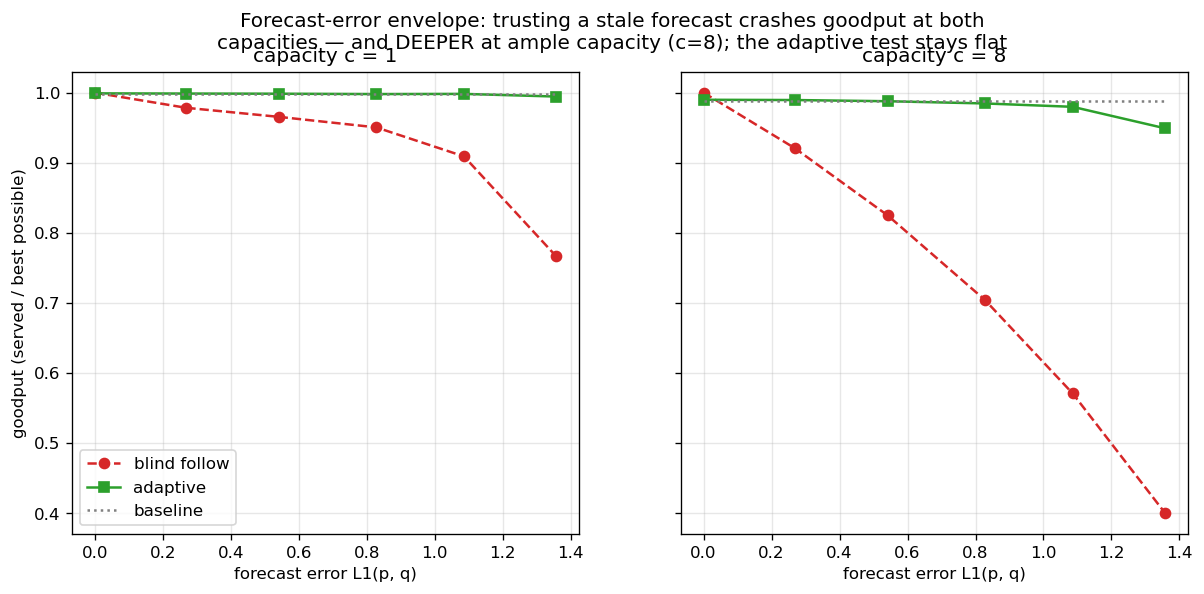
\includegraphics[width=0.7\linewidth,height=\textheight,keepaspectratio,alt={Capacity as robustness: blindly following the forecast crashes goodput --- deeper at ample capacity (c=8) --- while the adaptive test stays flat.}]{../../results/serving_envelope.png}
\caption{Capacity as robustness: blindly following the forecast crashes
goodput --- deeper at ample capacity (\(c=8\)) --- while the adaptive
test stays flat.}
\end{figure}

\textbf{Capacity as robustness} (\textbf{Figure 9.1}). Increasing the
capacity \(c\) smooths the effect of a bad prediction: a capacity-aware
baseline stays safe, while \emph{blindly} trusting a traffic forecast
degrades \emph{further} as capacity grows. Capacity is thus a
\emph{substitute} for algorithmic robustness --- the systems analogue of
the robustness-insurance thesis.

\begin{figure}
\centering
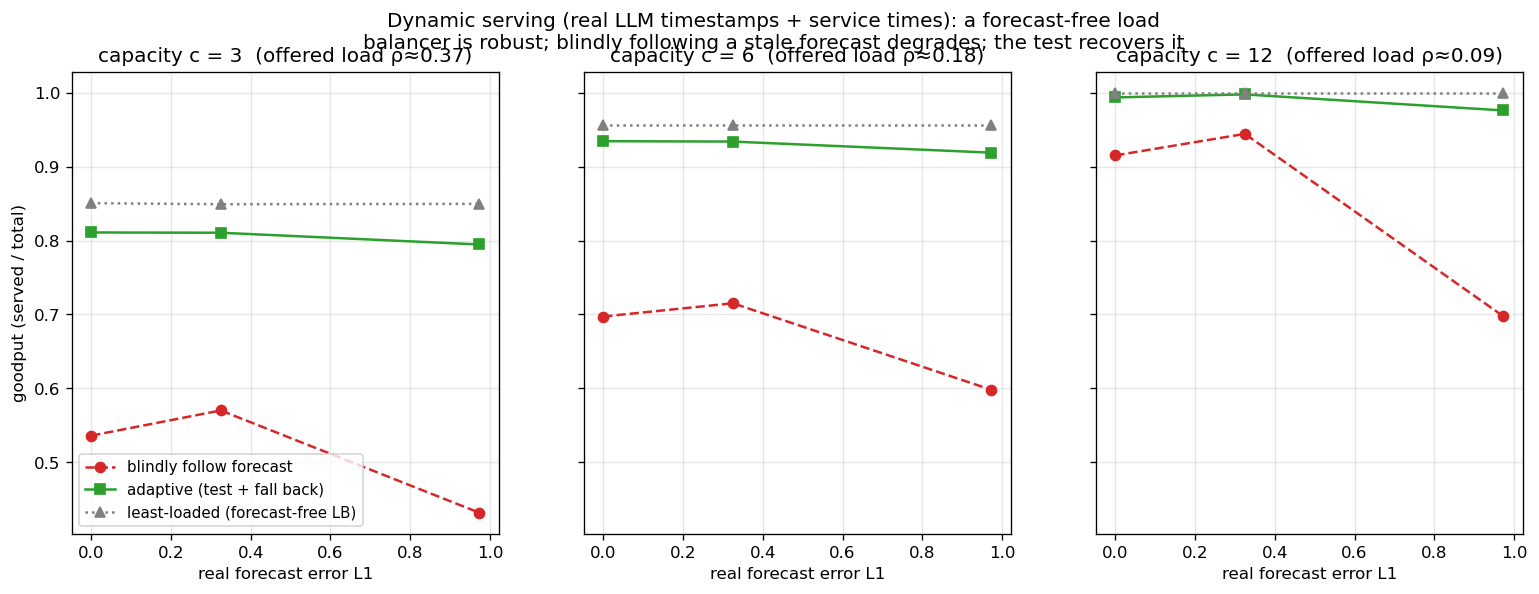
\includegraphics[width=1\linewidth,height=\textheight,keepaspectratio,alt={Live load beats a stale forecast under dynamic service times; an adaptive test recovers most of the gap.}]{../../results/serving_dynamic.png}
\caption{Live load beats a stale forecast under dynamic service times;
an adaptive test recovers most of the gap.}
\end{figure}

\textbf{Forecasts vs live load} (\textbf{Figure 9.2}). Under dynamic
service times (requests hold a slot for a real duration, released
event-by-event), a live-load signal beats a stale traffic forecast --- a
reactive load balancer outperforms a forecast-following router when the
forecast has aged.

\begin{figure}
\centering
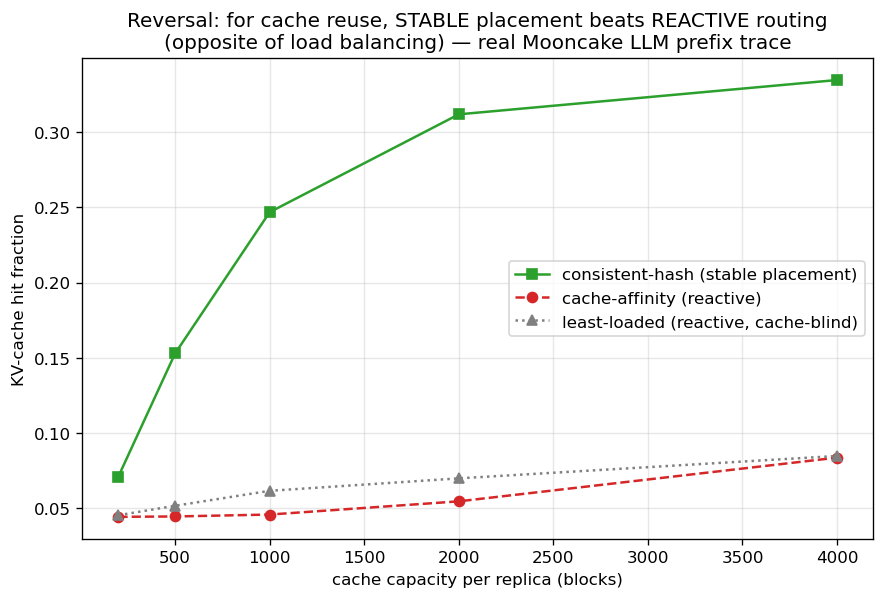
\includegraphics[width=0.6\linewidth,height=\textheight,keepaspectratio,alt={The cache-affinity reversal (Mooncake trace): stable placement beats reactive routing for KV-cache reuse.}]{../../results/prefix_cache_reversal.png}
\caption{The cache-affinity reversal (Mooncake trace): stable placement
beats reactive routing for KV-cache reuse.}
\end{figure}

\textbf{Cache-affinity routing} (\textbf{Figure 9.3}). For
prefix-cache-aware routing, a \emph{stable} affinity router beats a
reactive one --- the reverse of the traffic-forecast case, because cache
locality rewards persistence \autocite{preble2024}.

Each of these recovers an established systems result cleanly,
demonstrating that the framework instantiates the problem faithfully.

\section{A probe for a genuinely new result, and its
negative}

We also asked whether the with-predictions lens yields a \emph{new}
actionable serving result on a tail rather than a throughput objective.
It does not: on an SLO objective --- protecting a tight-SLO class of
requests under bursty load --- a non-predictive policy comes within
\(\le 3\%\) of one with perfect foresight across every regime swept. The
experiment, its caveats and its two explanations are in §8.2. The
consequence for this chapter is that we found no natural regime where
foresight helps, so serving remains a case study.

\section{Chapter summary}

The serving instantiation shows the framework reaches a live systems
problem and recovers its established results --- capacity as a
robustness substitute, live load over stale forecasts, stability for
cache locality --- and that even a tail objective does not open a
genuine with-predictions win.
